\problemname{Veggspjöld}
\illustration{0.4}{posters}{Veggspjöld}

\noindent
Hrolleifur er mikill kvikmyndaáhugamaður og safnar allskyns munum
tengdum kvikmyndum. Eitt af því sem hann hefur stundað er að safna
veggspjöldum sem auglýsa kvikmyndirnar. Hann hefur gætt þess að eiga
til að minnsta kosti eitt veggspjald fyrir hverja kvikmynd, sem hann
límir síðan á vegginn í herberginu sínu.

Nú hefur Hrolleifur safnað veggspjöldunum í fjölda ára og nálgast að
þau þekji vegginn hann fullkomlega. Eftir að Hrolleifur hefur límt veggspjald
situr það fast á sínum stað. Því miður hefur Hrolleifur ekki alltaf
verið nógu vandvirkur þegar hann límir þau á vegginn og því skarast
sum veggspjöldin þó svo að veggurinn sé ekki fullþakinn.

Veggur Hrolleifs og öll veggspjöldin eru rétthyrnd. Þó svo að
Hrolleifur hafi ekki alltaf gætt þess að láta veggspjöldin ekki 
skarast, hefur hann ávallt gætt þess að veggspjöldin snúi rétt,
því er efri brún veggspjaldanna ávallt lárétt.

Hve stórt svæði af veggnum er enn ónotað?

\begin{figure}[h!]
  \centering
    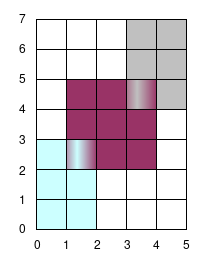
\includegraphics[width=0.5\textwidth]{sample2}
  \caption{Sýnidæmi 2}
\end{figure}

\section*{Inntak}
Fyrsta lína inniheldur þrjár heiltölur $b, h$ og $n$ þar sem
$b$ og $h$ eru breidd og hæð vegg Hrolleifs og $n$ er fjöldi
veggspjaldanna sem hann hefur límt á vegginn. Það gildir alltaf
að $1 \leq b,h \leq 10^9$ og $1 \leq n \leq 10^5$.
Næst fylgja $n$ línur með fjórum heiltölum hver,
$0 \leq x_1 < x_2 \leq b$ og $0 \leq y_1 < y_2 \leq h$ þar sem
$x_1$, $x_2$ eru fjarlægðir vinstri og hægri brúnar veggspjaldsins
frá vinstri hlið veggjarins og $y_1$, $y_2$ eru fjarlægðir neðri
og efri brúnar veggspjaldsins frá loftinu. Allar einingar eru 
í sentímetrum.

\section*{Úttak}
Skrifaðu út eina heiltölu, flatarmál þess hluta veggjarins sem er ekki þakið neinu veggspjaldi í fersentímetrum.

\section*{Stigagjöf}
\begin{tabular}{|l|l|l|l|}
\hline
Hópur & Stig & Takmarkanir \\ \hline
1     & 10    & $1 \leq b, h \leq 200$, $0 \leq n \leq 50$, engin tvö veggspjöld skarast \\ \hline % naive 
2     & 15   & $1 \leq b, h \leq 200$, $0 \leq n \leq 50$, mesta lagi tvö veggspjöld skarast á sama stað\\ \hline % naive + remove overlapping pairs
3     & 20   & $1 \leq b, h \leq 200$, $1 \leq n \leq 1\,000$  \\ \hline % O(nbh)
4     & 25   & $1 \leq b, h \leq 2\,000$, $1 \leq n \leq 1\,000$ \\ \hline % O(nb+bh) or O(nh+bh)
5     & 25   & $1 \leq n \leq 1\,000$ \\ \hline % O(n^2 log n)
6     & 5   & Engar frekari takmarkanir \\ \hline % O(n log n)
\end{tabular}
